% This file was created by matlab2tikz.
%
%The latest updates can be retrieved from
%  http://www.mathworks.com/matlabcentral/fileexchange/22022-matlab2tikz-matlab2tikz
%where you can also make suggestions and rate matlab2tikz.
%
\definecolor{mycolor1}{rgb}{0.00000,0.44700,0.74100}%
%
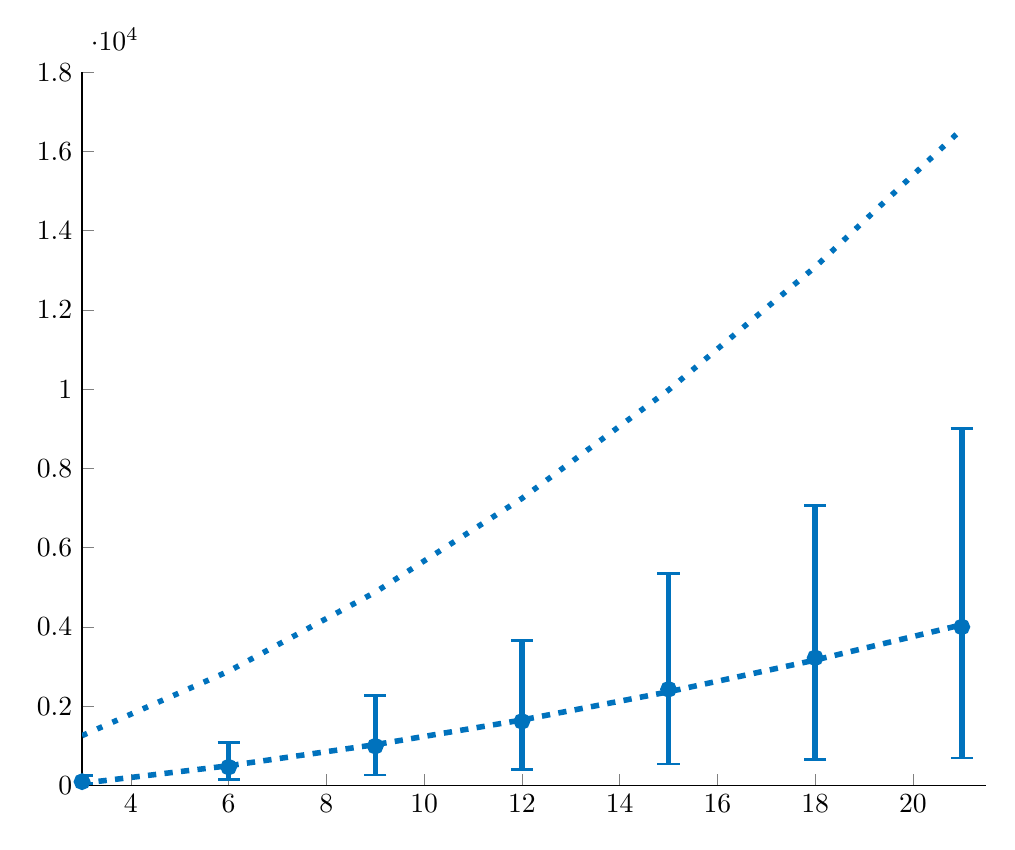
\begin{tikzpicture}

\begin{axis}[%
width=4.521in,
height=3.566in,
at={(0.758in,0.481in)},
scale only axis,
xmin=3,
xmax=21.5,
xlabel style={font=\color{white!15!black}},
%xlabel={m (column number)},
ymin=0,
ymax=18000,
ylabel style={font=\color{white!15!black}},
%ylabel={Time (seconds)},
axis background/.style={fill=white},
title style={font=\bfseries},
%title={$\text{Average ticks until solution as a function of m. On n }\times\text{ m grid. (k = 21)}$},
axis x line*=bottom,
axis y line*=left,
legend style={at={(0.03,0.97)}, anchor=north west, legend cell align=left, align=left, draw=white!15!black}
]
\addplot [color=mycolor1, draw=none, mark=*, mark options={solid, mycolor1}, line width=2pt]
  table[row sep=crcr]{%
3	92.795\\
6	459.7155\\
9	988.7515\\
12	1614.389\\
15	2424.197\\
18	3219.723\\
21	3998.259\\
};
%\addlegendentry{$\text{n = 18; T}_{\text{est}}\text{ = 0.276}\cdot\text{n}\cdot\text{m}^\text{2}\text{ + O(m)}$}

\addplot [color=mycolor1, loosely dotted, line width=2pt]%, forget plot]
  table[row sep=crcr]{%
3	1254.85714285714\\
6	2880\\
9	4875.42857142857\\
12	7241.14285714286\\
15	9977.14285714286\\
18	13083.4285714286\\
21	16560\\
};
\addplot [color=mycolor1, draw=none, line width=2pt, forget plot]
 plot [error bars/.cd, y dir = both, y explicit, error bar style={line width=2pt}, error mark options={line width=1pt,mark size=4pt,rotate=90}]
 table[row sep=crcr, y error plus index=2, y error minus index=3]{%
3	92.795	152	37\\
6	459.7155	624	304\\
9	988.7515	1280	729\\
12	1614.389	2040	1218\\
15	2424.197	2930	1884\\
18	3219.723	3836	2565\\
21	3998.259	5012	3306\\
};
\addplot [color=mycolor1, dashed, line width=2pt, forget plot]
  table[row sep=crcr]{%
3	51.447976190482\\
6	494.55767857143\\
9	1027.16425\\
12	1649.26769047619\\
15	2360.868\\
18	3161.96517857143\\
21	4052.55922619048\\
};
\end{axis}
\end{tikzpicture}%